\documentclass{article}


\usepackage[a4paper, includeheadfoot,margin=2cm]{geometry}
\usepackage{amsfonts}
\usepackage{amsmath}
\usepackage{graphicx}
\graphicspath{{./Images/}}
\usepackage{mathrsfs}
\usepackage{siunitx}
\usepackage{systeme}
\usepackage{textcomp}
\usepackage{xcolor}
\usepackage{wrapfig}
\usepackage{tikz}
\usepackage{MnSymbol}
\usepackage{tocbibind}
\usepackage[toc,page]{appendix}
\usepackage{titling}

\newenvironment{codeFont}{\fontfamily{pcr}\selectfont}{\par}
\newenvironment{gitFont}{\fontfamily{zi4}\selectfont}{\par}



\pretitle{

\begin{center}

\includegraphics[scale=0.45]{Polimi}

\bigskip
\bigskip
\bigskip
\bigskip
\bigskip
\bigskip
\bigskip


}
\posttitle{ \end{center}}




\begin{document}

\title{\Huge Prova Finale del Corso di Reti Logiche\\ \huge Politecnico di Milano}
\author{\Large Lorenzo Gadolini \and \Large Giuseppe Lischio.}
\date{}



\bigskip

\maketitle




\pagenumbering{Roman}

\newpage

\tableofcontents





\newpage
\pagenumbering{arabic}




\setcounter{page}{1}


\section{Introduzione}
\begin{flushleft}
Il metodo di codifica a Working-Zones propone un'ottimizzazione orientata alla riduzione del consumo di energia introdotto dall'input/output di un microprocessore.

\medskip

Sia dato un generico sistema composto da un processore e una memoria esterna al chip referenziabile tramite un bus indirizzi. Questo metodo suggerisce che un programma in esecuzione sul dato sistema sfrutti durante la sua esecuzione un insieme di indirizzi "preferiti", e che quindi sia più efficiente racchiudere tutti questi indirizzi dentro uno spazio di lavoro (detto appunto Working-Zone). 

\medskip

Gli indirizzi di queste Working-Zones sono codificati tramite un sistema base e offset, così da ridurre ulteriormente la quantità di informazione trasmessa sul bus indirizzi, e di conseguenza ridurre anche l'energia dissipata.

\end{flushleft}

\bigskip
\subsection{Dati Progettuali e Specifica}
\begin{flushleft}

Il componente da progettare ha come compito quello di stabilire se un indirizzo che riceve in input appartiene o meno ad una delle Working-Zones stabilite, e in caso affermativo di effettuare la traduzione dell'indirizzo da binario naturale a codifica WZE.

\medskip

Il componente si interfaccia con una memoria indirizzabile al byte a partire dall'indirizzo 0, e in cui vengono inizializzati i dati necessari per effettuare la computazione. La memoria inoltre è indirizzabile tramite indirizzi di 16 bit.

\medskip

Gli indirizzi di memoria da 0 a 7 contengono le basi delle 8 Working-Zones stabilite in fase di setup e scritte in binario naturale senza segno su 7 bit.
\smallskip

La cella di memoria 8 contiene l'indirizzo su cui effettuare la verifica e l'eventuale codifica, anch'esso scritto in binario naturale senza segno su 7 bit.
\smallskip

L'indirizzo di memoria 9 conterrà a fine computazione un numero di 8 bit senza segno, che come verrà descritto più avanti potrà essere una codifica o un indirizzo semplice.

\medskip

I restanti indirizzi sono tutti inizializzati a 0 e non vengono sfruttati durante la computazione.

\medskip

Gli indirizzi delle Working-Zones sono supposti non ripetuti, ed inoltre si suppone che non ci sia overlapping tra gli spazi delle varie Working-Zones. Per cui ogni indirizzo analizzato appartiene al più ad una Working-Zone.

\end{flushleft}

\bigskip
\subsection{La fase di traduzione}
\begin{flushleft}

Nella fase di codifica il componente deve essere in grado di stabilire se un indirizzo depositato nella cella numero 8 della memoria appartiene o meno ad una Working-Zone.

\medskip

Un indirizzo che non appartiene a nessuna Working-Zone fa entrare il componente in uno stato di "Non appartenenza", stato in cui la macchina secondo specifica deve depositare in uscita il dato così come le è stato fornito, preceduto da un bit posto a "0".
\smallskip

Il dato in uscita è un intero binario naturale senza segno di 8 bit.

\bigskip

\begin{gitFont}

"0" \& "0101010"  \ \  --Codifica\footnote{Il simbolo \& indica concatenazione di bit} esempio di indirizzo che non cade in alcuna WZ

\end{gitFont}



\newpage

Se il componente stabilisce che l'indirizzo appartiene ad una Working-Zone, scatta la fase di "Appartenenza", il dato necessita di encoding.


Un indirizzo codificato è un numero di 8 bit senza segno composto da tre sottogruppi di bit.

\begin{itemize}
\item Il bit più significativo viene posto ad "1", che indica "Codifica avvenuta";
\item I tre bit successivi codificano posizionalmente la Working-Zone a cui tale indirizzo appartiene. Il dato in uscita è un numero binario naturale senza segno da 0 a 7 che indica che l'indirizzo appartiene alla "n-esima" Working-Zone.



\item I quattro bit finali codificano l'offset dell'indirizzo dalla base. Il numero codificato è un numero binario One Hot. L'offset indica la distanza posizionale in memoria dall'indirizzo base, ovvero l'indirizzo "si trova a" n indirizzi dalla base.  %%Se si crea un appendice, spiegare la codifica one hot.
\end{itemize}

\bigskip


\begin{gitFont}

"1" \& " 010" \& " 0100"  \ \ --Codifica esempio di indirizzo appartenente ad una WZ

\end{gitFont}


\bigskip

Sia che l'indirizzo appartenga o che non appartenga ad una Working-Zone, il componente prosegue sempre lungo la stessa fase di output. Il dato viene depositato in memoria, salvato, e la macchina entra in fase di attesa di reset e/o avvio per una successiva codifica.
\end{flushleft}
\subsubsection{Entity del componente}

Il componente hardware è stato descritto tramite linguaggio VHDL in base alle specifiche fornite dal tema di progetto.

La struttura input/output del componente in VHDL è stata fornita nelle specifiche ed è di seguito riportata.


\begin{center}
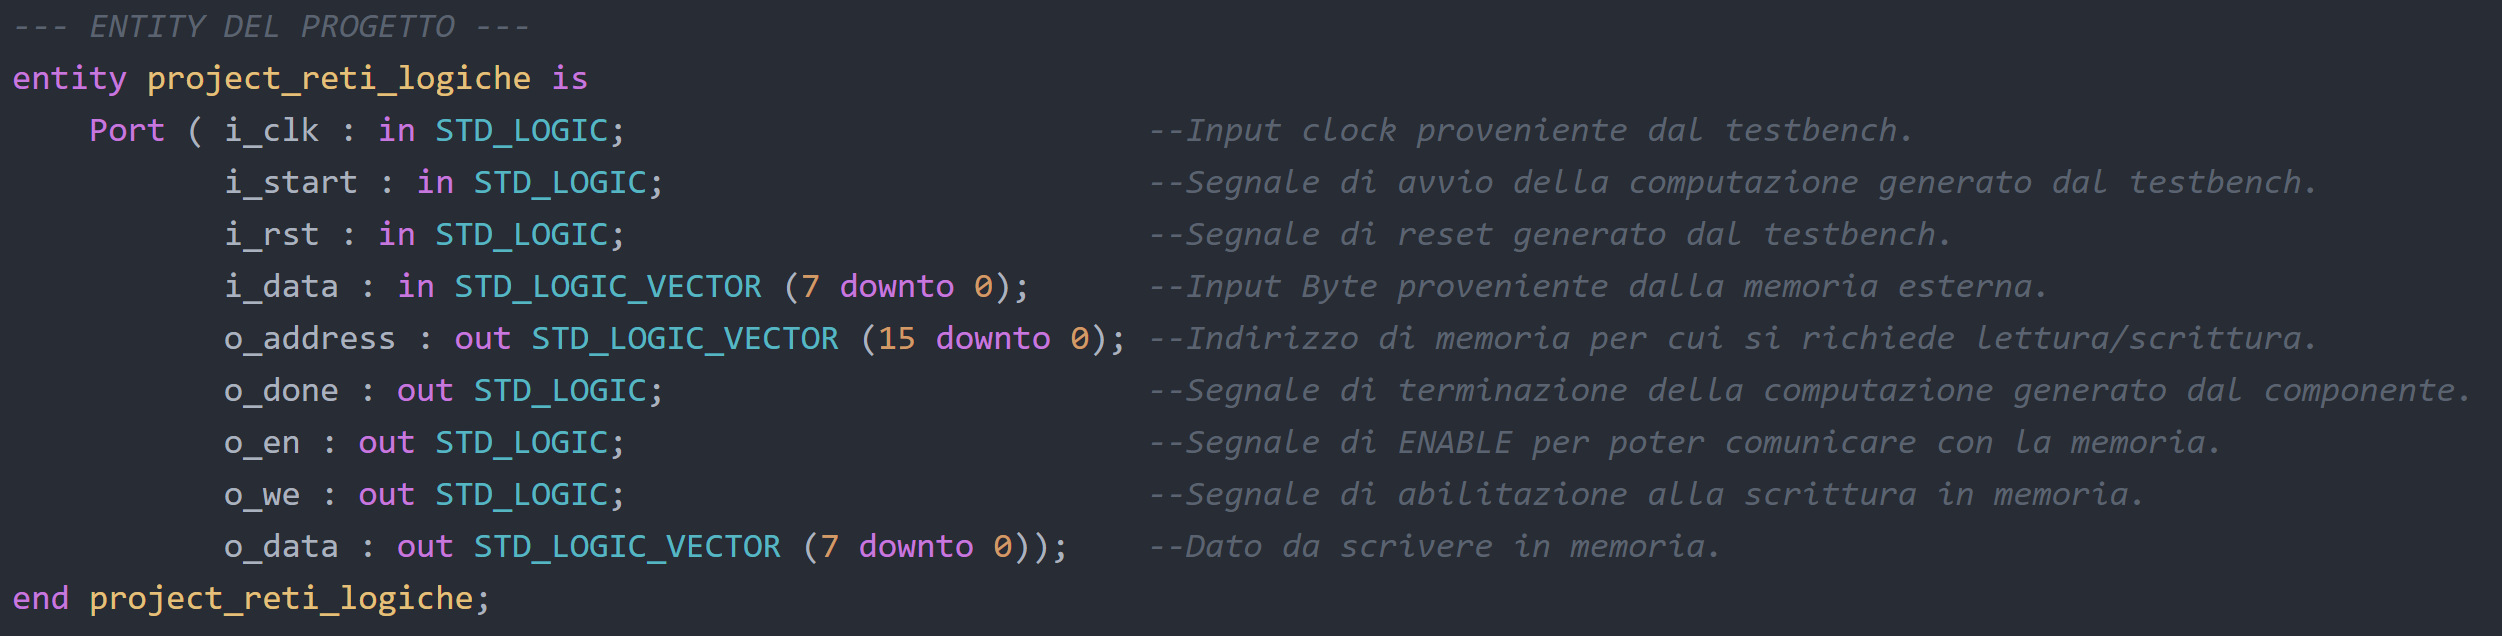
\includegraphics[scale=0.27]{Entity}
\end{center}

\bigskip
\bigskip

\begin{center}
\line(1,0){350}
\end{center}

\newpage

\section{Architettura e Scelte Progettuali}

\bigskip

\subsection{L'algoritmo}

\begin{flushleft}


Il progetto si basa su un algoritmo alquanto semplice.
\smallskip

Dato uno stato iniziale di memoria, per prima cosa viene letto il dato di cui si necessita la codifica dall'indirizzo di memoria numero 8, successivamente il componente entra in un ciclo di calcolo. In questo ciclo di calcolo vengono letti uno alla volta i byte di memoria 0-7 contenenti gli indirizzi base delle Working zones.
\smallskip

 Il componente sottrae l'indirizzo da codificare all'indirizzo base letto, e verifica che il risultato cada fra 0 e 3. Questo risultato ha il significato di offset, e come da specifica, un offset compreso fra 0 e 3 (inclusi) indica un'appartenenza alla Working-Zone. Qualsiasi altro risultato viene interpretato come "Non appartenenza".

\bigskip

\subsection{Non Appartenenza}\label{notA}

Un risultato che non appartiene a nessuna Working-Zone deve venire propagato in uscita così come è stato letto da memoria in entrata. Il componente ha terminato gli otto cicli di verifica e ha determinato che l'indirizzo in input non appartiene a nessuna Working-Zone. A questo punto la macchina carica i 7 bit dell'indirizzo nel registro di output, il quale era stato inizializzato con 8 bit tutti posti a zero, così da rispettare la specifica che prevede di emettere in uscita uno 0 seguito dai 7 bit dell'indirizzo scritti in binario naturale senza segno.

\bigskip

\subsection{Appartenenza}\label{app}

Se il componente durante la sua esecuzione verifica che l'indirizzo da codificare cade all'interno di una delle basi, allora si avvia la procedura di encoding. Per prima cosa viene codificato l'offset. Il risultato della sottrazione appartiene ad un insieme finito e ristretto di valori, per questo si è scelto di creare una Lookup Table che contenesse tali valori di offset già tradotti in codifica OneHot. La macchina si occupa di assegnare al valore di uscita uno dei valori di offset tradotti.
Una volta scritto in memoria il primo quartetto di bit, il componente passa alla traduzione della tripletta di bit contenente l'indirizzo della Working-Zones. Questa fase scrive i tre bit che corrispondono al valore binario naturale del byte di memoria che contiene l'indirizzo base nel registro di out.

Infine il componente pone ad 1 il MSB del valore di uscita, cosi che chi riceve il valore tradotto a valle riconosce che è stato effettuato l'encoding.



\end{flushleft}

\newpage

\subsection{Il design: La macchina a stati}

Il progetto del componente parte dalla descrizione di una macchina a stati che esegua l'algoritmo sopra enunciato.

La macchina a stati completa che esegue la codifica è disegnata qui:

\begin{flushleft}
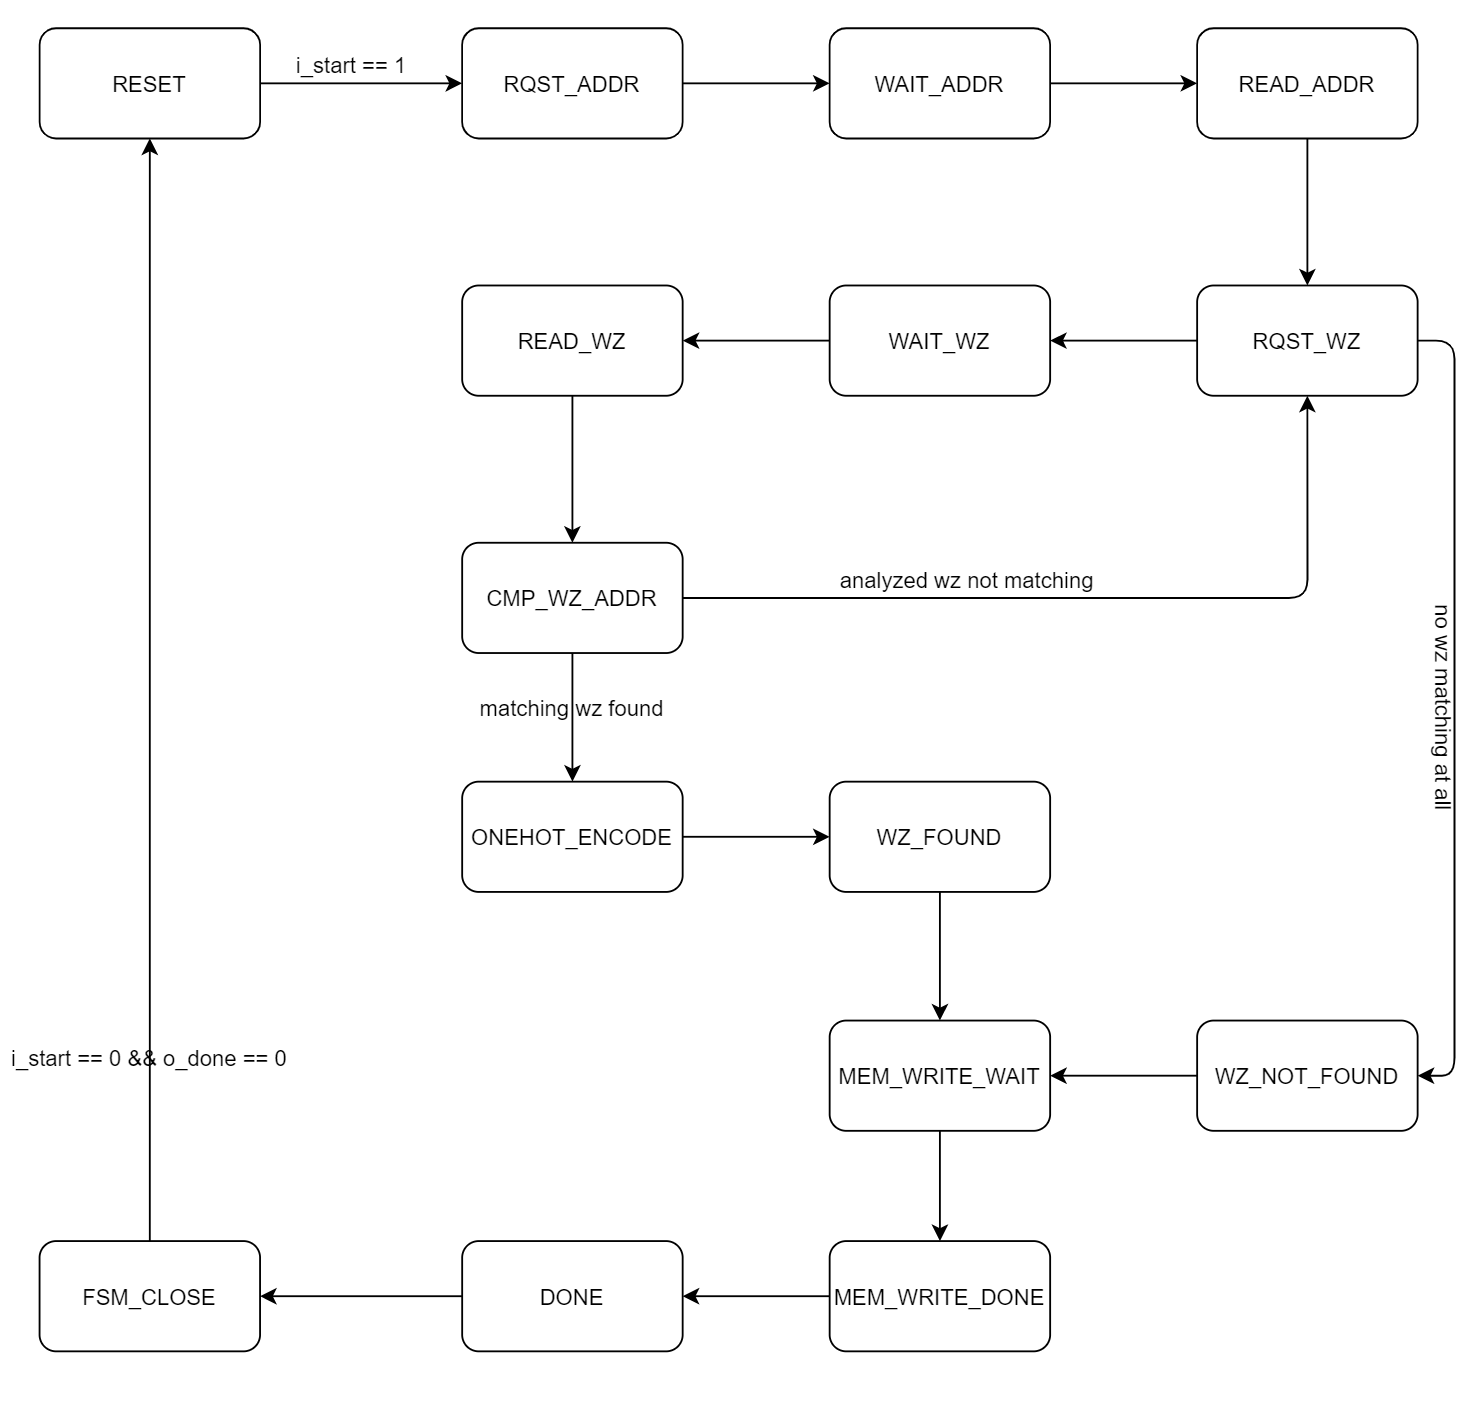
\includegraphics[scale=0.45]{FSM}
\end{flushleft}

Nel paragrafo \ref{fsm} verranno specificati i compiti dei singoli stati e delle transizioni.

\newpage

\subsubsection{Descrizione degli stati}\label{fsm}

\begin{itemize}

\item RESET: Lo stato in cui la macchina viene avviata e a cui giunge una volta che riceve il segnale di reset o che termina una computazione. La macchina cicla su questo stato attendendo un segnale di start. Successivamente inizializza la memoria e salta al primo vero stato di esecuzione.

\item RQST\_ ADDR: La macchina richiede alla memoria l'indirizzo da codificare.

\item WAIT\_ ADDR: La macchina attende per un ciclo di clock la propagazione dei segnali alla memoria.

\item READ\_ ADDR: La macchina ottiene il dato dalla memoria.

\item RQST\_ WZ: La macchina richiede alla memoria il valore della n-esima base, dove n è compreso fra 0 e 7.

\item WAIT\_ WZ: La macchina attende un ciclo di clock la propagazione dei segnali alla memoria.

\item READ\_ WZ: La macchina ottiene la base n-esima dalla memoria.

\item CMP\_ WZ\_ ADDR: La macchina esegue la sottrazione che determina l'appartenenza o meno e l'offset del dato da codificare.

\item ONEHOT\_ ENCODE: La macchina codifica l'offset di un indirizzo che ha dato esito positivo in una comparazione.

\item WZ\_ FOUND: La macchina prepara il byte contenente il dato codificato e notifica alla memoria che è pronto per essere scritto.

\item WZ\_ NOT\_ FOUND: La macchina notifica alla memoria che il dato non appartiene a nessuna Working-Zone, e che è pronta a propagarlo senza codifica.

\item MEM\_ WRITE \_ WAIT: La macchina attende un ciclo di clock che la memoria riceva la sua richiesta di scrittura.

\item MEM\_ WRITE\_ DONE: La macchina completa la fase di scrittura.

\item DONE: La macchina notifica il raggiungimento dello stato di terminazione portando il segnale di completamento ad '1'.

\item FSM\_ CLOSE: La macchina attende che il segnale di avvio torni a '0' per poter portare a '0' il segnale di completamento e successivamente passare allo stato di reset per avviare un'eventuale computazione successiva.

\end{itemize}

\begin{flushleft}


Nel grafico della macchina è stato escluso l'autoanello dello stato di reset. L'autoanello è necessario perchè permette alla macchina di rimanere in attesa su tale stato che il segnale di avvio torni ad '1', iniziando una nuova computazione.
\smallskip

Nel grafico per lo stesso motivo è stato escluso l'autoanello sullo stato FSM\_ CLOSE. La macchina in tale stato attende ciclando sull'autoanello che il segnale di avvio vada a '0'.

 Sono stati inoltre esclusi tutti gli archi che da ogni singolo stato portano allo stato di reset.
\begin{gitFont}i{\_}rst \end{gitFont} potrebbe venire posto ad '1' in qualsiasi momento della computazione. 
\smallskip

Data questa evenienza è necessario che la macchina, in qualsiasi stato si trovi, abbandoni l'encoding ed entri nello stato di reset. 
\smallskip

Questo si ottiene con una gestione asincrona della verifica del segnale. 
Ad ogni ciclo di clock viene analizzato tale segnale, e se riscontrato ad '1' la macchina esegue una transizione dallo stato in cui si trova a RESET.

\end{flushleft}

\subsection{Il Codice VHDL}

\begin{flushleft}

In questo piccolo paragrafo viene fatta un'analisi di come è stata descritta la macchina a stati in linguaggio VHDL, analizzandone i segnali e i registri necessari al funzionamento.

Il componente è stato descritto tramite codice VHDL Behavioral che implementa tutti gli stati elencati nel paragrafo \ref{fsm}.

 Oltre all'architettura fornita dalla specifica, il componente possiede altri segnali e registri che si sono resi necessari in fase di scrittura di codice.

\begin{flushleft}
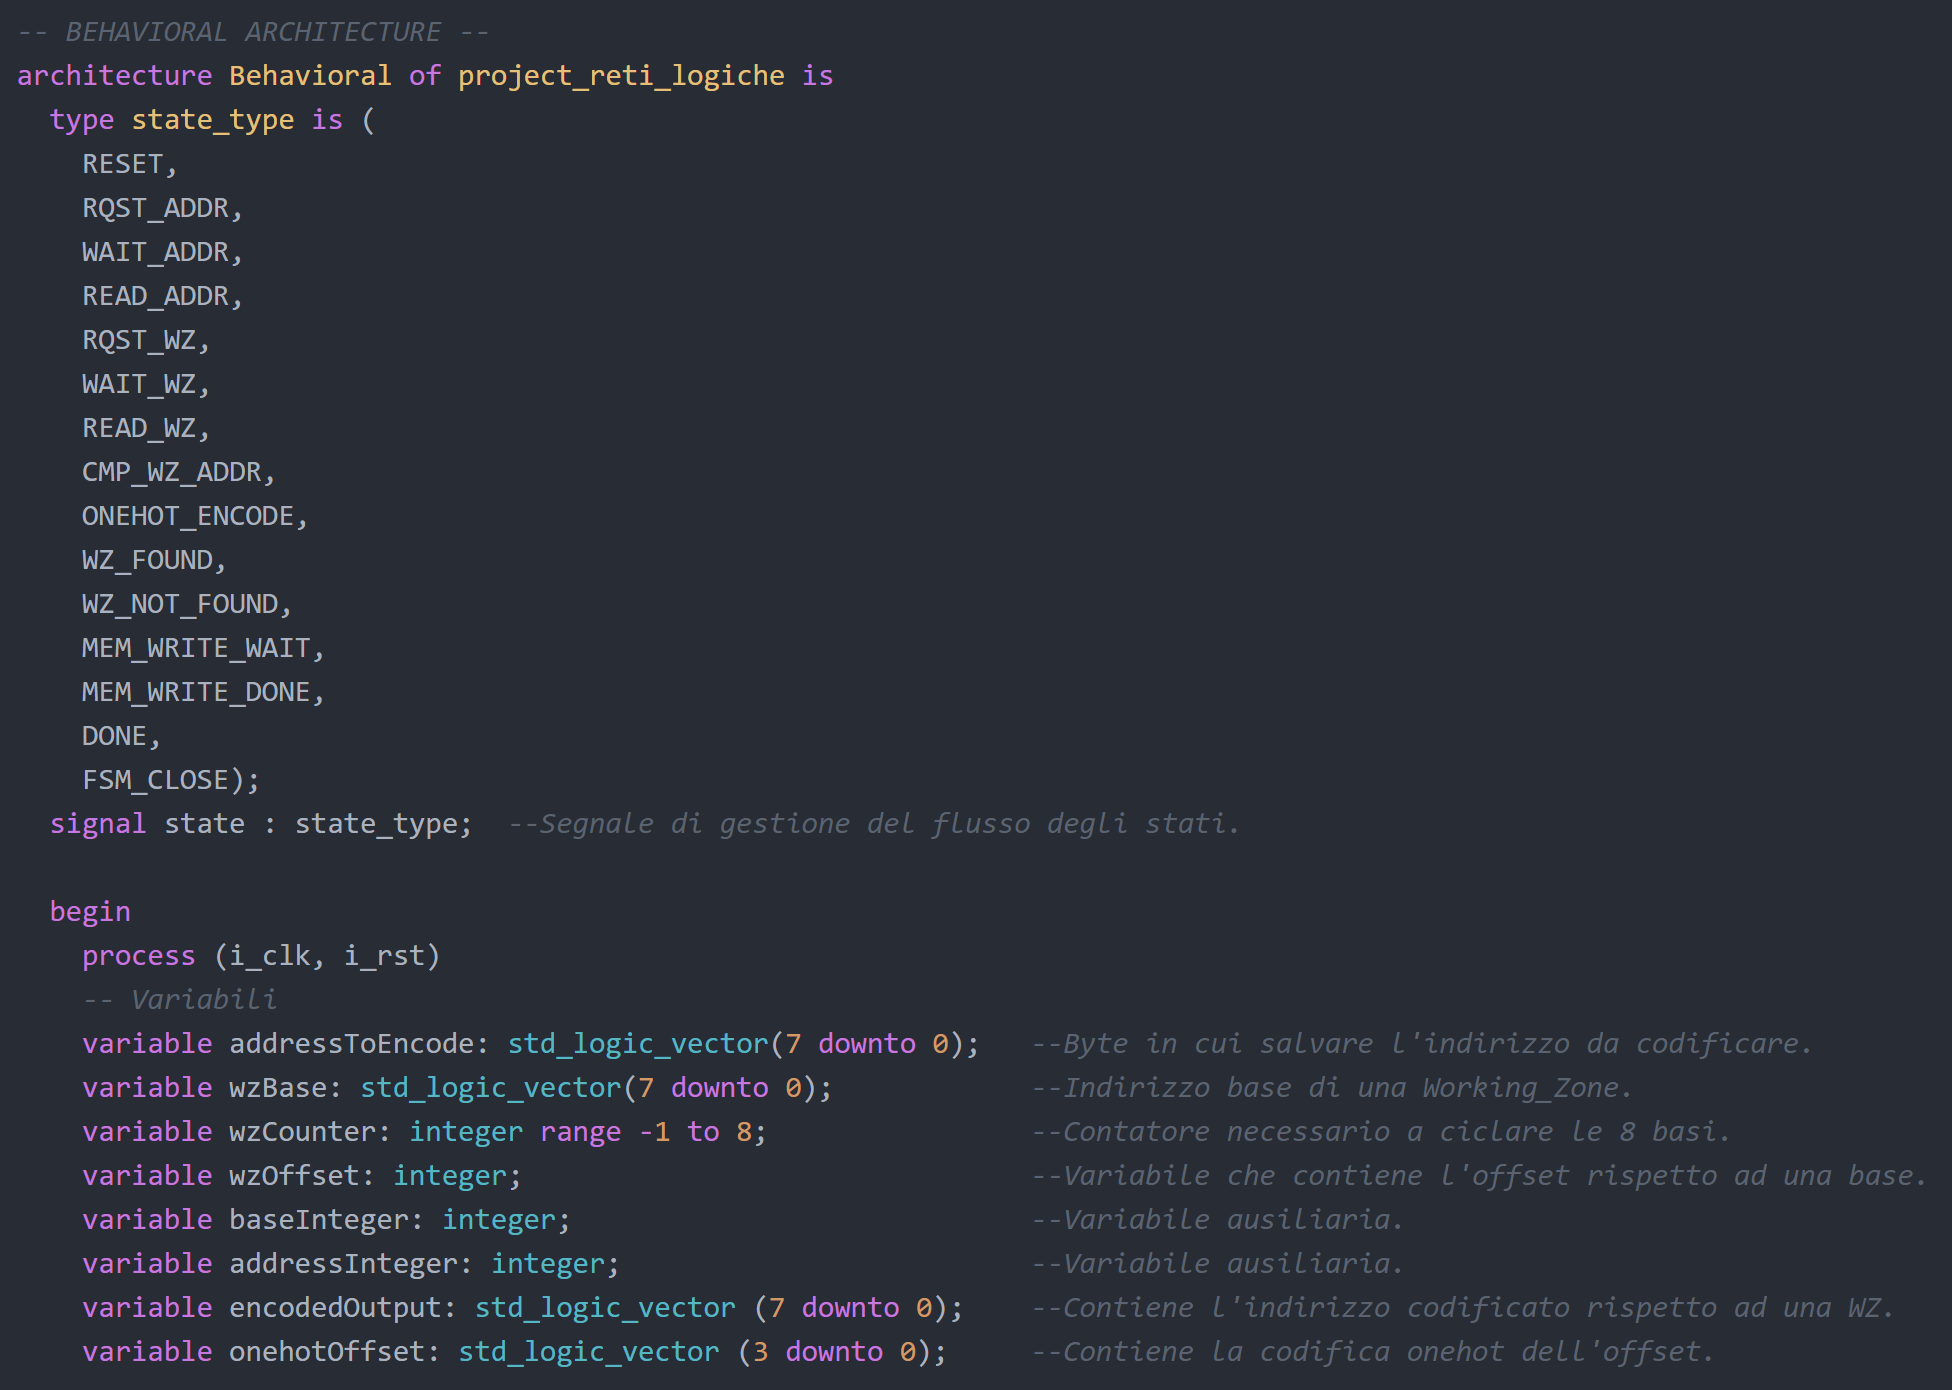
\includegraphics[scale=0.31]{Behavioral}
\end{flushleft}


\begin{itemize}

\item \begin{gitFont}
addressToEncode
\end{gitFont} Variabile di tipo std{\_}logic{\_}vector a 8 bit, viene utilizzata per salvare l'indirizzo che necessita di valutazione e codifica.

\item \begin{gitFont}
wzBase
\end{gitFont} Variabile std{\_}logic{\_}vector a 8 bit che salva nel ciclo di computazione la base della Working-Zone e viene aggiornata ad ogni risultato di non appartenenza con la base successiva.

\item \begin{gitFont}
wzCounter
\end{gitFont} Variabile integer che  può assumere valori da -1 (default) ad 8. Viene sfruttata come flag per segnalare a quale valore di byte in memoria siamo arrivati. Raggiunto il valore 8 funge da flag per segnalare al componente che non ci sono più Working-Zones da valutare e che la macchina deve entrare in stato di "Non Appartenenza" (par. \ref{notA}).

\item \begin{gitFont}
wzOffset
\end{gitFont} Variabile integer che salva il valore dell'offset di un indirizzo rispetto alla sua base in caso la macchina determini che tale indirizzo appartiene ad una Working-Zone.

\item \begin{gitFont}
encodedOutput
\end{gitFont} Variabile di tipo std{\_}logic{\_}vector a 8 bit che salva un indirizzo che è stato sottoposto a processo di encoding ( par. \ref{app}).

\item \begin{gitFont}
encodedOutput
\end{gitFont} Variabile di tipo std{\_}logic{\_}vector a 4 bit che viene sfruttata dalla macchina per salvare il valore di offset in codifica OneHot.

\end{itemize}

\end{flushleft}

\bigskip




\begin{center}
\line(1,0){350}
\end{center}

\bigskip
\bigskip
\section{Risultati della Sintesi}
Il componente progettato è stato sintetizzato in maniera virtuale tramite l'apposito tool di Vivado. Come FPGA target è stata utilizzata una Xilinx xc7a200tfbg484-1. La sintetizzazione ha dato un risultato positivo, ed il componente è stato testato con successo sia con test Behavioral che Post-Synthesis, con gli stessi test effettuati per il solo funzionamento logico. È emerso che il componente funziona correttamente anche impostando periodi di clock molto inferiori al requisito minimo della specifica (100 ns). Il report post sintesi di Vivado ha inoltre rilevato le seguenti percentuali di utilizzo delle risorse della FPGA utilizzata: 
\bigskip

\begin{center}
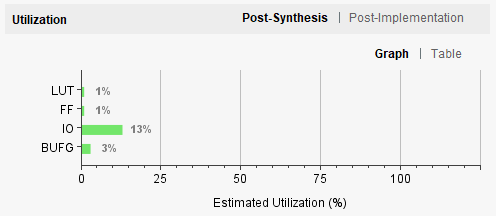
\includegraphics[scale=0.8]{postSynthesisUtilization} \\
\end{center}


\bigskip
\bigskip

\begin{center}
\line(1,0){350}
\end{center}

\newpage

\section{Simulazioni}

In questo paragrafo verranno discussi i metodi utilizzati per verificare il corretto funzionamento del componente progettato. In particolare è stato usato il software Xilinx "Vivado" per scrivere i test bench e per effettuare vari tipi di simulazione:

\begin{itemize}

\item Simulazione \textbf{Behavioral}: test del funzionamento logico, basato sul codice VHDL scritto, senza passare per la sintesi virtuale del componente.

\item Simulazione \textbf{Post-Synthesis Functional}: test che permette di verificare il comportamento strutturale del componente descritto. Viene eseguito dopo aver terminato il processo di sintesi virtuale.

\item Simulazione \textbf{Post-Synthesis Timing}: test analogo al \textit{Post-Synthesis Functional}, che tiene però conto di tutti i ritardi introdotti dalle porte logiche usate nella simulazione del componente virtuale.

\end{itemize}

\subsection{Test Benches}

Le tipologie di simulazione descritte sopra, sono state applicate su casi di test scritti ad hoc, per individuare eventuali punti deboli del funzionamento del componente. I test a cui la macchina è stata sottoposta sono:

\begin{itemize}

\item Test Bench singolo: test analogo a quello fornito dal personale docente, che sottopone alla macchina un singolo caso di test, per poi terminare.

\item Test Bench sequenziale: vengono sottoposti alla macchina dei casi di test da effettuare in maniera sequenziale. Per effettuare questo tipo di test, si è pensato di aggiungere al test bench singolo una gestione dei valori in input tramite un file di testo, contente un caso di test per ogni riga. La macchina, dopo aver terminato la computazione ed aver riportato il segnale \textit{tb{\_}done} a '0', riceve un segnale creato ad hoc, chiamato \textit{load{\_}ram}, grazie al quale viene fatta partire la lettura di un nuovo caso di test dal file, i cui valori vengono copiati in memoria, e con i quali viene eseguita una nuova computazione. In questo modo si è potuto verificare che la macchina non ha problemi con il reset dei segnali e delle celle di memoria. Inoltre è stato possibile testare la macchina su decine di migliaia di casi di test diversi, generati automaticamente tramite degli appositi script. 
%%qui c'è da inserire la foto e evidenziare il fatto che c'è un segnale di load ram che carica la nuova sequenza di valori presi dal file

\item Test Bench reset asincrono: viene testata la capacità della macchina di gestire un reset asincrono durante l'esecuzione di casi di test sequenziali. In particolare durante l'esecuzione di un caso di test, e dopo un intervallo di tempo prefissato, viene portato ad '1' il segnale di reset senza attendere che la macchina abbia terminato la sua fase di calcolo. 

\end{itemize}



\newpage
\subsection{Screenshots}


\paragraph{Simulazione Behavioral sequenziale}
Durante l'esecuzione di più casi di test consecutivi, si può notare come a seguito della memorizzazione del risultato computato, e dopo l'abbassamento - in questo caso contemporaneo - dei segnali \textit{tb{\_}done} e \textit{tb{\_}start}, il segnale \textit{load{\_}ram} venga portato ad '1' per consentire la lettura dei nuovi dati e poter cominciare un nuovo ciclo di computazione.
 
\begin{flushleft}
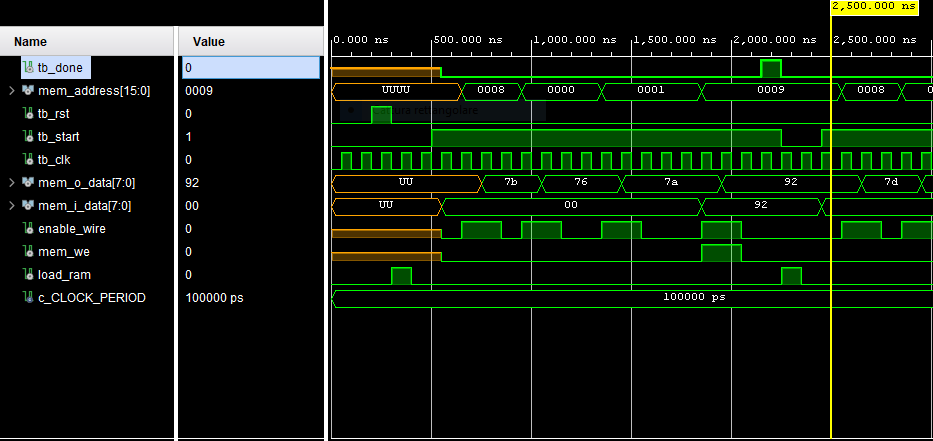
\includegraphics[scale=0.70]{dettaglio_behavioral} \\
\end{flushleft}

\bigskip
\paragraph{Simulazione Post-Synthesis Timing 5ns}\label{fast}
La macchina riesce ad effettuare la computazione anche con cicli di clock di durata 5ns. Si può notare come tra i fronti di discesa di \textit{tb{\_}done} e \textit{tb{\_}start} ci sia un piccolo ritardo di quasi un periodo di clock, dovuto alla rete combinatoria utilizzata per la sintesi virtuale del componente.

\begin{flushleft}
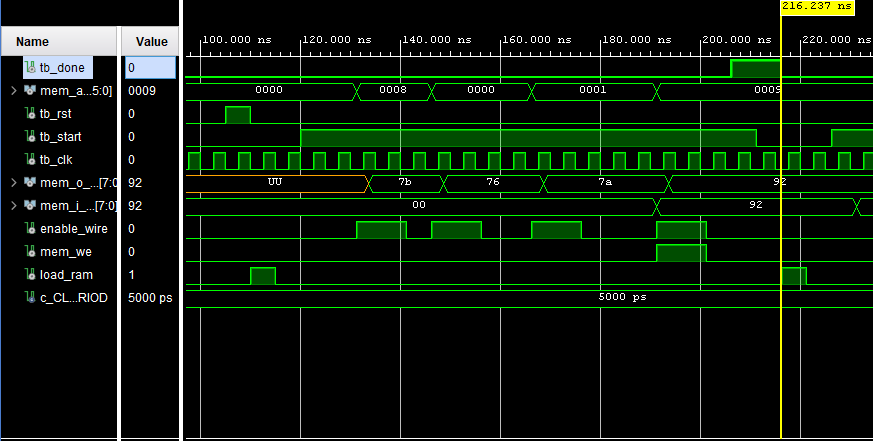
\includegraphics[scale=0.75]{dettaglio_postSynthesisTiming_5ns} \\
\end{flushleft}


\paragraph{Simulazione Behavioral, Reset Asincrono}

L'innalzamento del segnale di reset durante l'esecuzione di una computazione viene gestito correttamente dalla macchina. Nel dettaglio, dopo aver ricevuto tale segnale , la macchina è in grado di riavviare la computazione interrotta e giungere al termine del caso di test. Ciò accade perchè il segnale di reset ripristina la macchina ma non la memoria del testbench, per cui i dati letti restano identici all'esecuzione precedentemente interrotta.

\begin{flushleft}
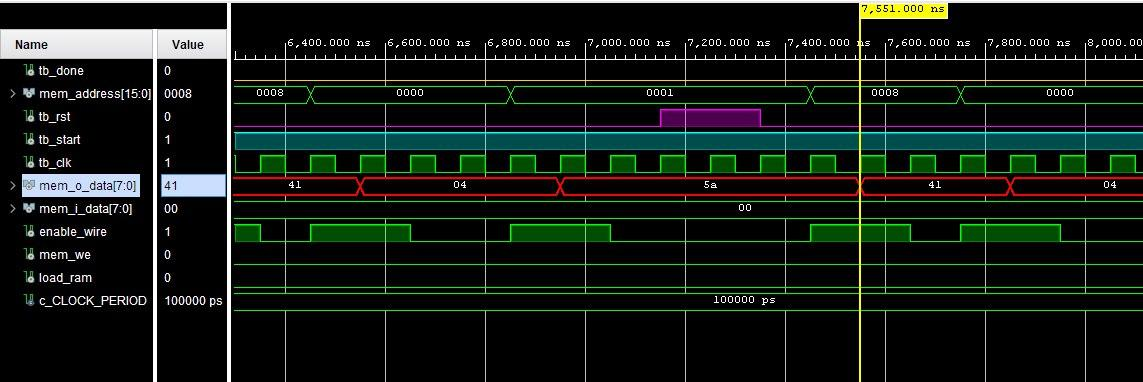
\includegraphics[scale=0.53]{Rst_Async} \\
\end{flushleft}

\bigskip

\begin{center}
\line(1,0){150}
\end{center}

\bigskip


\paragraph{Codice Test Bench Sequenziale}
%
Qui di seguito si trovano alcuni snippet del codice del test bench sequenziale, opportunamente commentato.
\begin{flushleft}
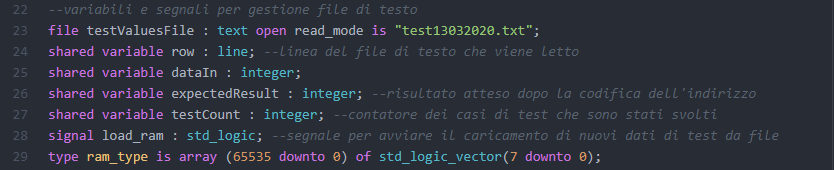
\includegraphics[scale=0.75]{sequential1} \\
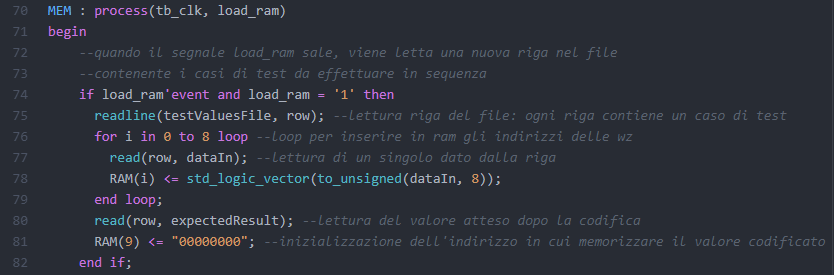
\includegraphics[scale=0.75]{sequential2} \\
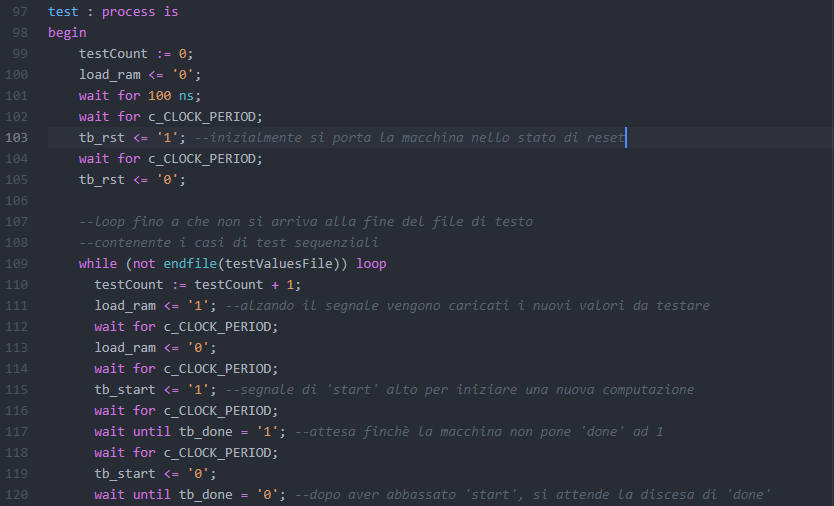
\includegraphics[scale=0.75]{sequential3} \\
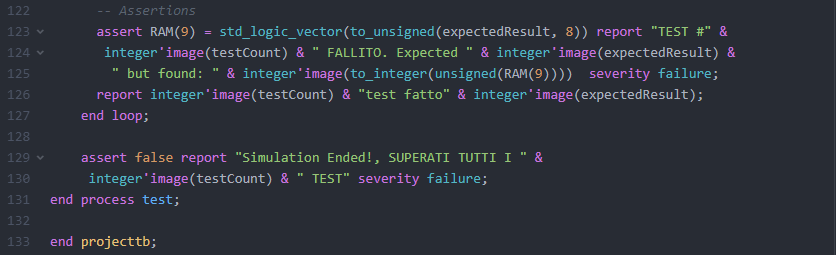
\includegraphics[scale=0.75]{sequential4} \\
\end{flushleft}

\bigskip
\bigskip


\begin{center}
\line(1,0){450}
\end{center}



\newpage


\section{Conclusioni}
L'algoritmo presentato come soluzione al problema ha complessità di calcolo al più lineare col numero di indirizzi che si presentano in ingresso. Questa affermazione si può dedurre dal fatto che l'automa ha un numero finito di stati (da cui il nome "FSA", finite state automata) che vengono percorsi un numero finito di volte anche se ciclicamente.

\smallskip

Il componente descritto è stato simulato in differenti situazioni di test che vanno dal caso semplice ad interruzioni impreviste della computazione, e anche se sottoposto a questi edge case è stato in grado comunque di portare a termine il suo compito.

\smallskip

Nel paragrafo \ref{fast} si analizza un caso di test in cui si sottopone una sintesi di componente a periodi di clock 20 volte più brevi rispetto alla specifica. Durante le fasi di test Post Synthesis Timing si è cercato un limite inferiore per la durata di un periodo di clock che non inficiasse l'esecuzione di una codifica, e questo limite si è scoperto aggirarsi attorno ai 3950 \emph{ps}.




























\end{document}
